\subsection{Ponte di Wheatstone}
Con il ponte "bilanciato" per il valore $R_x=R_{x0}$ si mostrano in figura \ref{fig:sbil} a titolo di esempio l'output dello "sbilanciamento" che il circuito mostra per diversi valori di $R_{x0}+\delta R_x$ e le misure ripetute sulla stessa configurazione a ponte bilanciato.\\
\begin{figure}[H]
    \centering
    \begin{minipage}{0.49\textwidth}
        \centering
        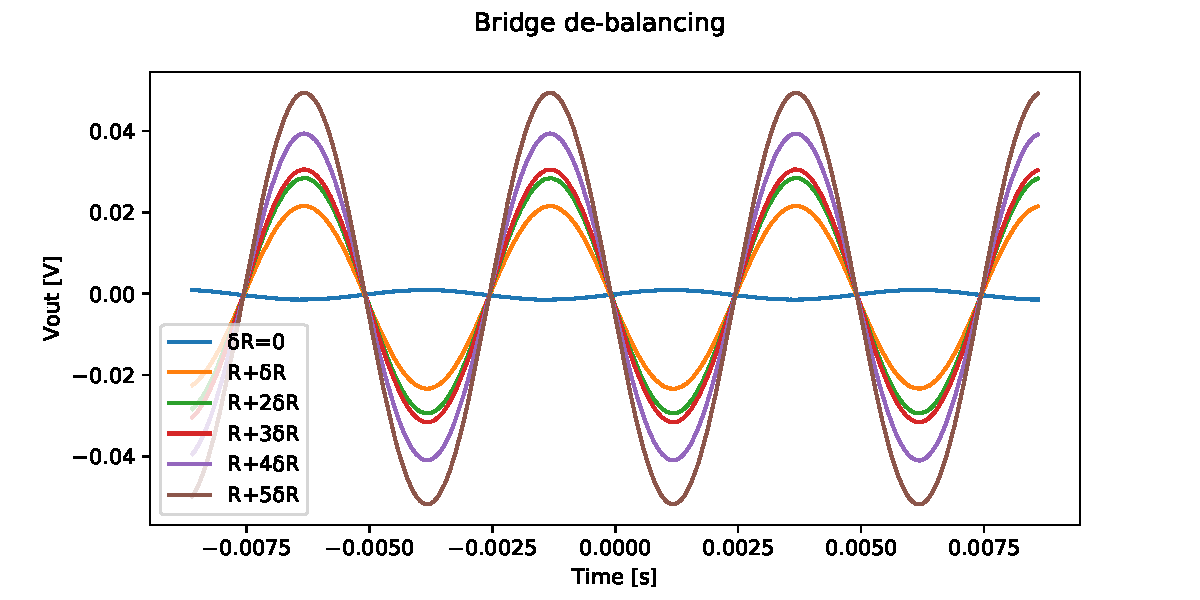
\includegraphics[width=\textwidth]{Figure_12.pdf}
    \end{minipage}\hfill
    \begin{minipage}{0.49\textwidth}
        \centering
        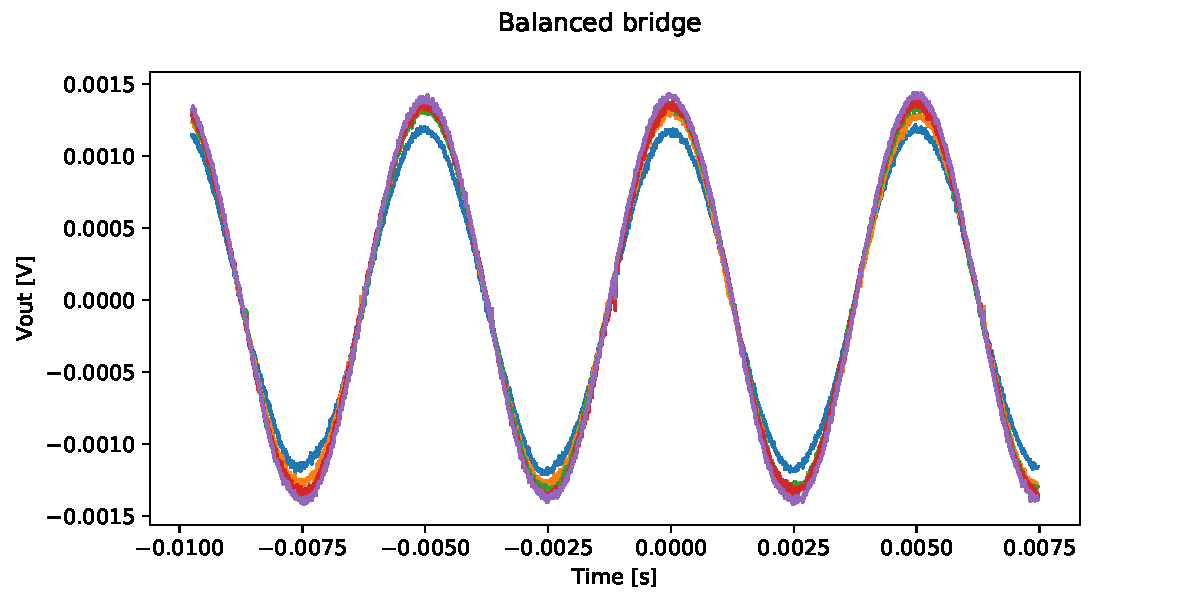
\includegraphics[width=\textwidth]{Figure_18.pdf} 
    \end{minipage}
    \caption{Sbilanciamento allontanandosi da $R_{x0}$ e misure ripetute a ponte bilanciato.}
    \label{fig:sbil}
\end{figure}
Le forme d'onda salvate utilizzando l'oscilloscopio, in modalit\'a 8 averagings, sono state date in input ad una funzione che esegue il fit sinusoidale alla frequenza che era impostata fornendo in output i parametri $A$, $B$ e $V_0$:
\begin{gather}
	V(t)=V_0+A \cos (\omega t)+B \sin (\omega t)
\end{gather}
Tuttavia per l'analisi \'e comodo che il segnale in ingresso sia un coseno puro in modo che il coefficiente $B$ tenda a zero, per fare questo i tempi vengono quindi traslati di un fattore comune sia in ingresso che in uscita partendo da un fit preliminare eseguito sull'ingresso:
\begin{gather}
	\phi=-\arctan (B/A) \\
	t_0=-\frac{\phi}{\omega} \\
	t \rightarrow t-t_0
\end{gather}
I coefficienti $A$ e $B$ possono essere riassunti da un unico numero immaginario trascurando il bias DC $V_0$ in modo che:
\begin{gather}
	V_{in}(t)=V_{0\ in}+V_{in}\cos (\omega t) \\
	V_{out}(t)=V_{0\ out}+A\cos (\omega t)+B\sin (\omega t)= V_{0\ out}+C \cos (\omega t+\phi) =\\
	\nonumber V_{0\ out}+C\cos (\phi)\cos (\omega t) -C \sin (\phi) \sin (\omega t) \\
	\mathbf{Re}[V_{out}]=A=C\cos (\phi) \\
	\mathbf{Im}[V_{out}]=-B=-C\sin (\phi) \\
	V_{out}=A-jB
\end{gather}
Quindi per ogni misurazione effettuata si ottengono due coppie di coefficienti $A$ $B$, una per l'ingresso e una per l'uscita.
Sulle misure ripetute nelle stesse condizioni (5 nel nostro caso) viene eseguita la media aritmetica dei valori e presa come incertezza la deviazione standard diviso $\sqrt{5}$.\\
Vengono quindi mostrati in figura \ref{fig:complan} gli effetti delle piccole variazioni di impedenza sulla risposta del ponte di misura.
\begin{figure}[h]
	\centering
    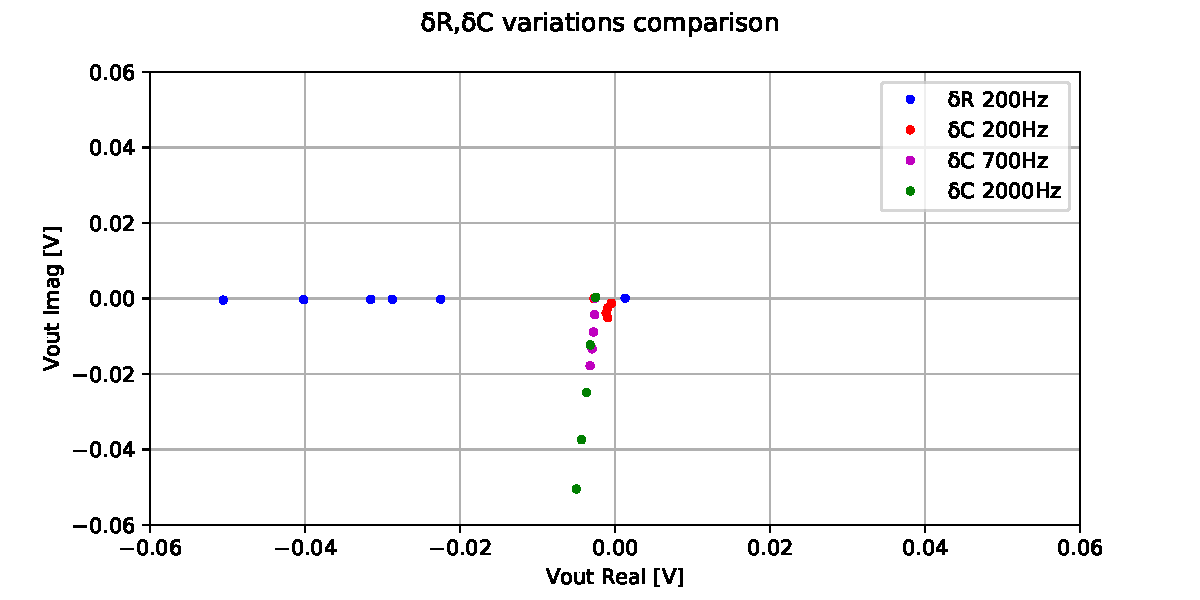
\includegraphics[width=\textwidth]{Figure_7.pdf}
    
    \caption{Plot di $V_{out}$ misurata sul piano immaginario.}
    \label{fig:complan}
\end{figure}
Si vede dalla figura come l'aggiunta di una componente puramente passiva non modifica sensibilmente la fase in uscita mentre se possiede componenti reattive l'effetto su $V_{out}$ \'e quello di uno sfasamento rappresentato da componenti immaginarie prominenti rispetto a quelle reali.\\
Per discriminare ulteriormente gli effetti si procede ad analizzare i vari casi separatamente.
\begin{figure}[h]
    \centering
    \begin{minipage}{0.5\textwidth}
        \centering
        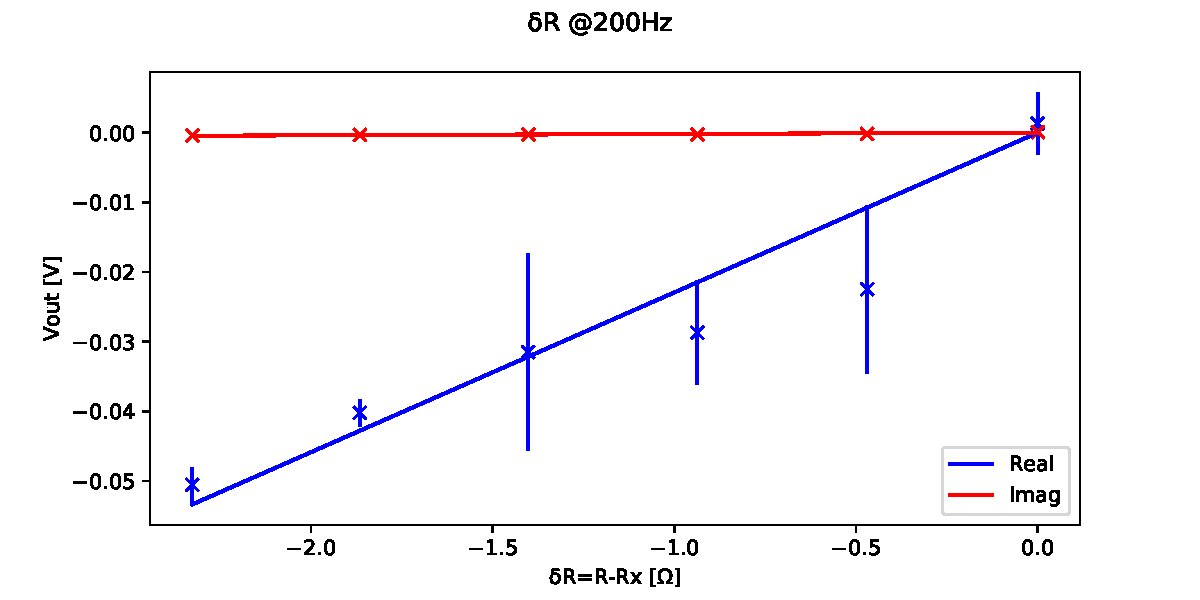
\includegraphics[width=\textwidth]{Figure_8.pdf} 
        %\caption{first figure}
    \end{minipage}\hfill
    \begin{minipage}{0.5\textwidth}
        \centering
        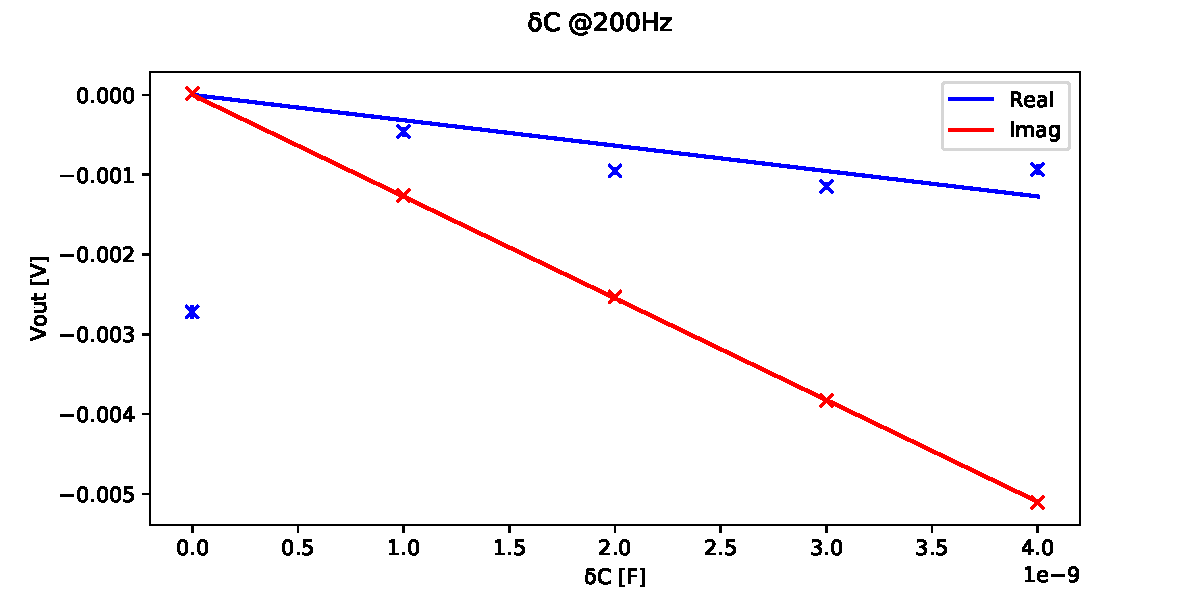
\includegraphics[width=\textwidth]{Figure_9.pdf} 
        %\caption{second figure}
    \end{minipage}
    \\
    \centering
    \begin{minipage}{0.5\textwidth}
        \centering
        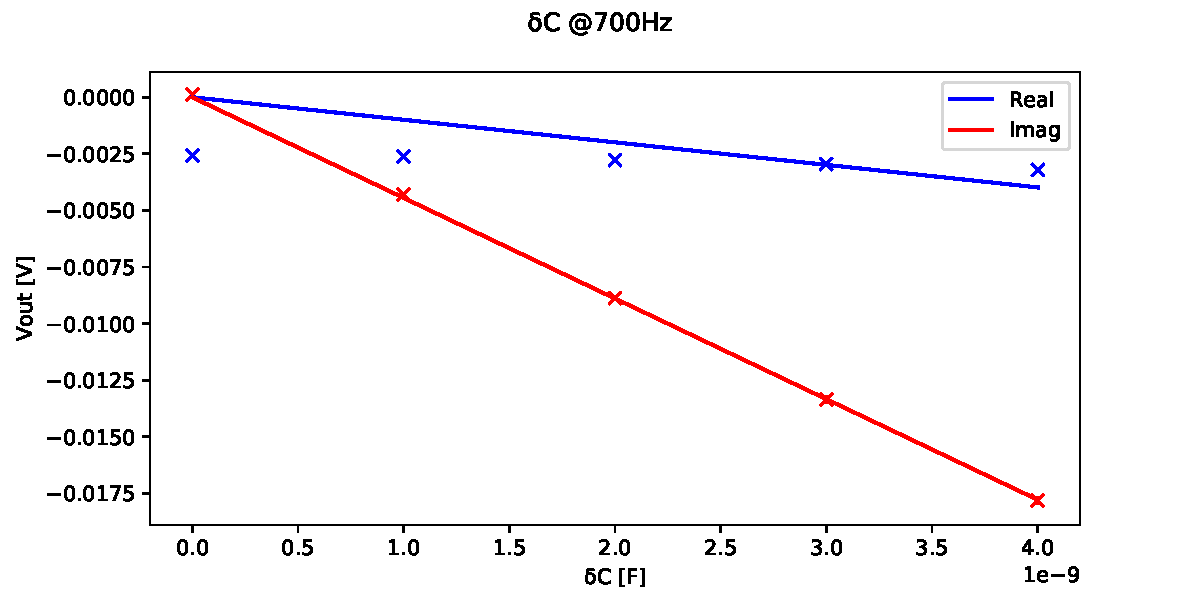
\includegraphics[width=\textwidth]{Figure_10.pdf} 
        %\caption{first figure}
    \end{minipage}\hfill
    \begin{minipage}{0.5\textwidth}
        \centering
        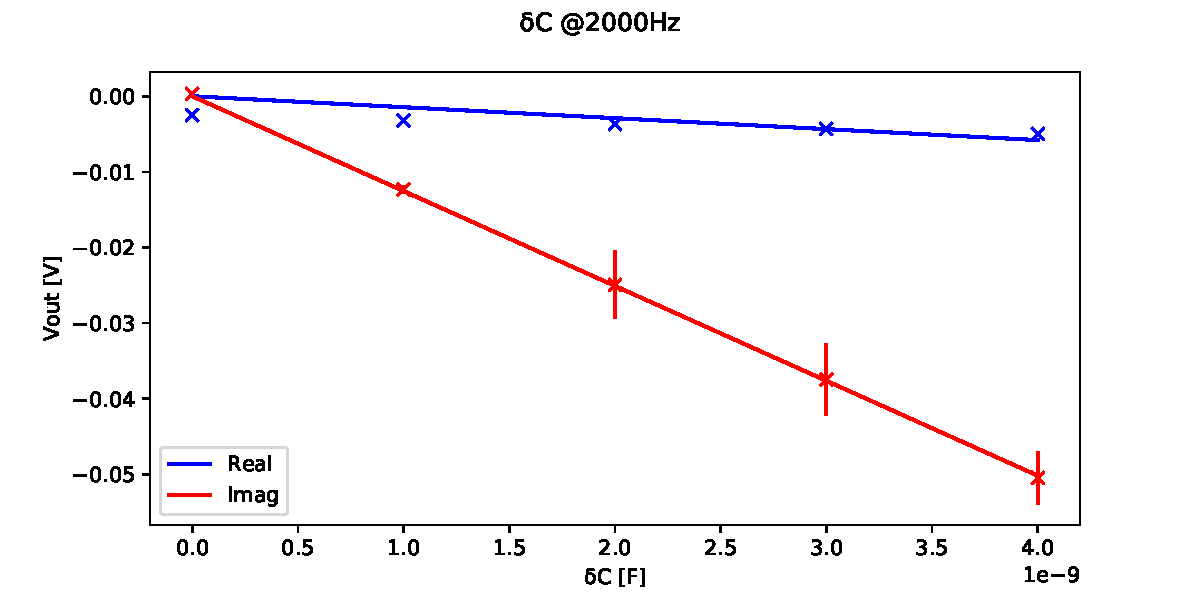
\includegraphics[width=\textwidth]{Figure_11.pdf} 
        %\caption{second figure}
    \end{minipage}
    \caption{$V_{out}$ in funzione di $\delta Z_x$}
    \label{fig:deltaz}
\end{figure}
Per ogni set di dati si procede ad effettuare una regressione lineare del tipo:
\begin{gather}
	\mathbf{Re}[V_{out}]=B \delta R_x \qquad \text{or}\\
	\mathbf{Im}[V_{out}]=B \delta C_x
\end{gather}
E si ottengono i risultati seguenti:
\begin{gather}
	\frac{\partial \mathbf{Re}[V_{out}]}{\partial \delta R_x} = 0.022934+/-0.000013 \ \si{\ampere} \\
	\frac{\partial \mathbf{Im}[V_{out}]}{\partial \delta C_x} = (-1.274+/-0.004)\E{6} \ \si{\volt\per\farad} \ @ \  200 \ \si{\hertz}\\
	\frac{\partial \mathbf{Im}[V_{out}]}{\partial \delta C_x} = (-4.4456+/-0.0010)\E{6} \ \si{\volt\per\farad} \ @ \  700 \ \si{\hertz}\\
	\frac{\partial \mathbf{Im}[V_{out}]}{\partial \delta C_x} = (-1.25414+/-0.00029)\E{7} \ \si{\volt\per\farad} \ @ \  2000 \ \si{\hertz}
\end{gather}
Tuttavia i $\chi^2_{red}$ sono rispettivamente $3343$, $0.9$, $790$ e $22981$ i quali non mostrano compatibilit\'a con la teoria se non nel secondo caso, si procede quindi ad assumere una sottostima delle incertezze che vengono quindi ampliate di conseguenza imponendo $\chi^2_{red}=1$ come \'e gi\'a stato mostrato nei plot in figura \ref{fig:deltaz}. Si ottengono quindi i valori (precedenti) con le nuove incertezze:
\begin{gather}
	\frac{\partial \mathbf{Re}[V_{out}]}{\partial \delta R_x} = 0.0229+/-0.0007 \ \si{\ampere} \\
	\frac{\partial \mathbf{Im}[V_{out}]}{\partial \delta C_x} = (-1.27+/-0.10)\E{6} \ \si{\volt\per\farad} \ @ \  200 \ \si{\hertz}\\
	\frac{\partial \mathbf{Im}[V_{out}]}{\partial \delta C_x} = (-4.4456+/-0.0010)\E{6} \ \si{\volt\per\farad} \ @ \  700 \ \si{\hertz}\\
	\frac{\partial \mathbf{Im}[V_{out}]}{\partial \delta C_x} = (-1.25+/-0.04)\E{7} \ \si{\volt\per\farad} \ @ \  2000 \ \si{\hertz}
\end{gather}

Si procede ora ad effettuare il calcolo della sensibilit\'a del circuito, ovvero la minima variazione di $\delta Z_x$ che esso \'e in grado di risolvere. \\
\begin{gather}
	\sigma_{\delta R} = \frac{ \sigma[\mathbf{Re}[V_{out}]] }{ \frac{\partial \mathbf{Re}[V_{out}]}{\partial \delta R_x}} = 0.6\ \si{\ohm} \\
	\sigma_{\delta C}=\frac{\sigma [\mathbf{Im}[V_{out}]]}{\frac{\partial \mathbf{Im}[V_{out}]}{\partial \delta C_x}} = 1\E{-11} \ \si{\farad} \ @ \  200 \ \si{\hertz} \\
	\sigma_{\delta C}= 2\E{-11} \ \si{\farad} \ @ \  700 \ \si{\hertz} \\
	\sigma_{\delta C}= 1.3\E{-11} \ \si{\farad} \ @ \  2000 \ \si{\hertz}
\end{gather}
